\chapter{Animasjoner, lyd og brukertilpasning}
 
 
 
\section{Animasjon} 
 
 
I denne prototypen skjer animasjonene som en respons på at brukeren trykker på et symbol. Hva som skjer avhenger av hvilken type symbol det er. De ulike typene som finnes i symboltabellen ble forklart i kapittelet om Sono flex, og er ordsymbol, kategorisymbol og navigasjonssymbol. Med Animasjonene vil en først og fremst gi brukeren tilbakemelding om at et valg har blitt gjort, men de skal også gjøre programvaren mer spennende.  I Sono Flex vil ingen av knappene ha noe visuelt som gjør at brukeren kan skille hva som skjer, utenom at symboltabellen bytter ut de eksisterende symbolene. I dette tilfelle vil en se at symbolet går fra å være et statisk symbol til å bli flyttet til setningslisten og bli en del av ønsket setning.  
  
 
 
\subsection{Animasjoner: ordsymbol} 
 

Når en bruker trykker på et ordsymbol, vil symbolet legge seg i setningslisten og er da klar for gjøres om til tydelig tale. Når brukeren har fullført setningen i Sono Flex blir brukeren presentert for endringen ved at symbolet vises i setningsfeltet. Med prototypen ønsker vi  å gi en mer visuell representasjon av denne endringen til brukeren. Ved å la brukeren kunne velge mellom to animasjoner som oppstår når han trykker på ønsket ordsymbol. 

\subsubsection{Glide animasjon}
Den ene animasjonen er vist i figur \ref{fig:OrdAnimasjon} og viser \textit{Glide Animasjonen}. I tilfelle med figuren under har brukeren akkurat trykket på brikken hvor det står "oksefrosk". Det dukker så opp en brikke som er identisk med den han trykket på. Denne brikken begynner så å gli i en rett linje mot målet, som er første posisjon i setningslisten. Hadde det allerede vært en brikke i listen ville den ha tatt høyde for dette og animasjonen tilpasset seg. 
 
 
 \begin{figure}
 \centering
 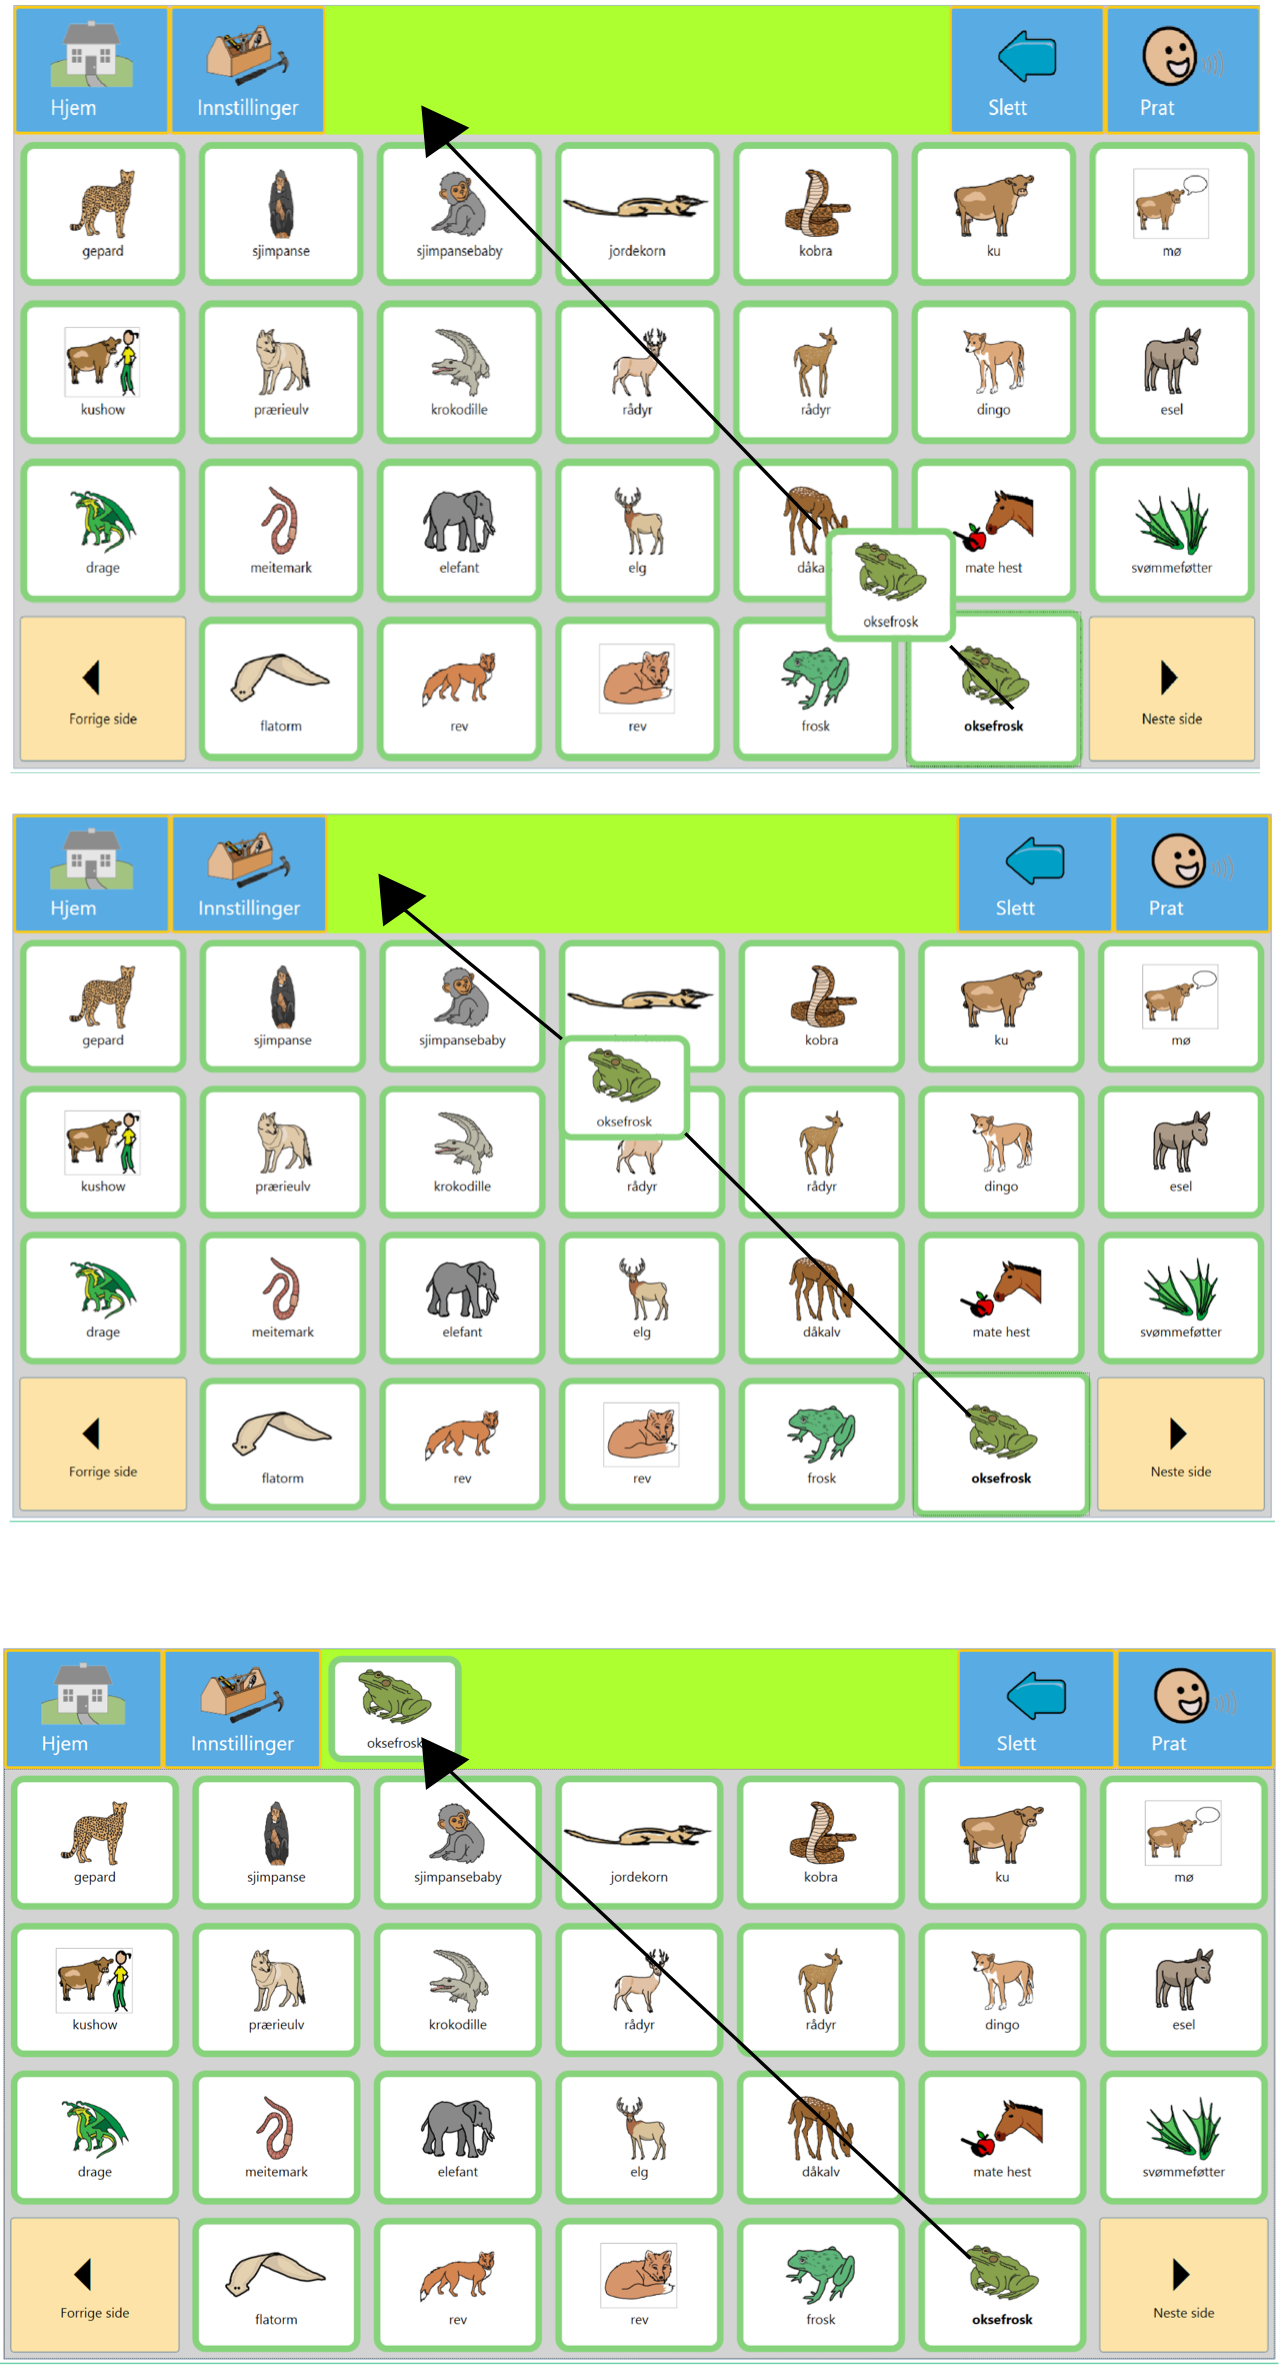
\includegraphics[height=18cm,keepaspectratio]{Frogs}
 \caption{Langt Bilde}
 \label{fig:OrdAnimasjon}
 \end{figure}


\subsubsection{Minimer - Maksimer}

Den andre animasjonen 

   Ordsymbolet krympes til 5 prosent av størrelsen. 
   I setningslisten vil en kopi av det krympede ordsymbolet dukke opp. 
   Kopien forstørres så til den opprinnelige størrelsen. 
   Ordsymbolet som opprinnelige ble trykket blir forstørret til opprinnelig størrelse. 
 

\subsection{Animasjon: Kategorisymbol} 
 
 
Når en bruker trykker på et kategorisymbol vil symbolene i symboltabellen byttes ut med symbolene som hører til i den gjeldene kategorien. Hvis en trykker på kategorien "dyr" så vil tabellen fylles med ordsymbol som "Hund", "katt", "tiger" o.s.v. Her ønsker animasjonen å hjelpe til med å fortelle at man ikke trykker på ordet dyr, men kategorien dyr og at brukeren får en forståelse for forskjellen mellom dem. Animasjonen startet ved at symbolet som brukeren trykket på forstørres helt til den dekker hele symboltabellen. Det vil si at ingen av de andre symbolene vises, kun kategorisymbolet. Symbolet vil så igjen forminskes, men symbolene i tabellen vil være erstattet av symbolene som tilhører kategorien.  
 
 
 
 
\subsection{Animasjon: Navigasjonssymbol} 
 
 
Den siste typen symbol er navigasjon og ved interaksjon vil den navigere mellom sider når det ikke er plass til alle symbolene på en side. Det vil si at symbolet skal kunne navigere fremover, fra side 1 til 2 og 2 til 3 og bakover igjen. 

Figur \ref{fig:navAni} viser hva som skjer fra brukeren trykker på neste side nede i høyre hjørne. Når brukeren trykker fremover starter animasjonen ved at alle symbolene som er på gjeldene side og neste side begynner å bevege seg mot venstre. Slik at symbolene på gjeldene side kontinuerlig blir byttet ut med de på neste. Symbolene på siden sklir ut, mens symbolene på neste sklir inn og overtar plassene. Når brukeren nå trykker på bakover-symbolet vil det samme skje bare at symbolene sklir mot høyre. 
 

\begin{figure}
\centering
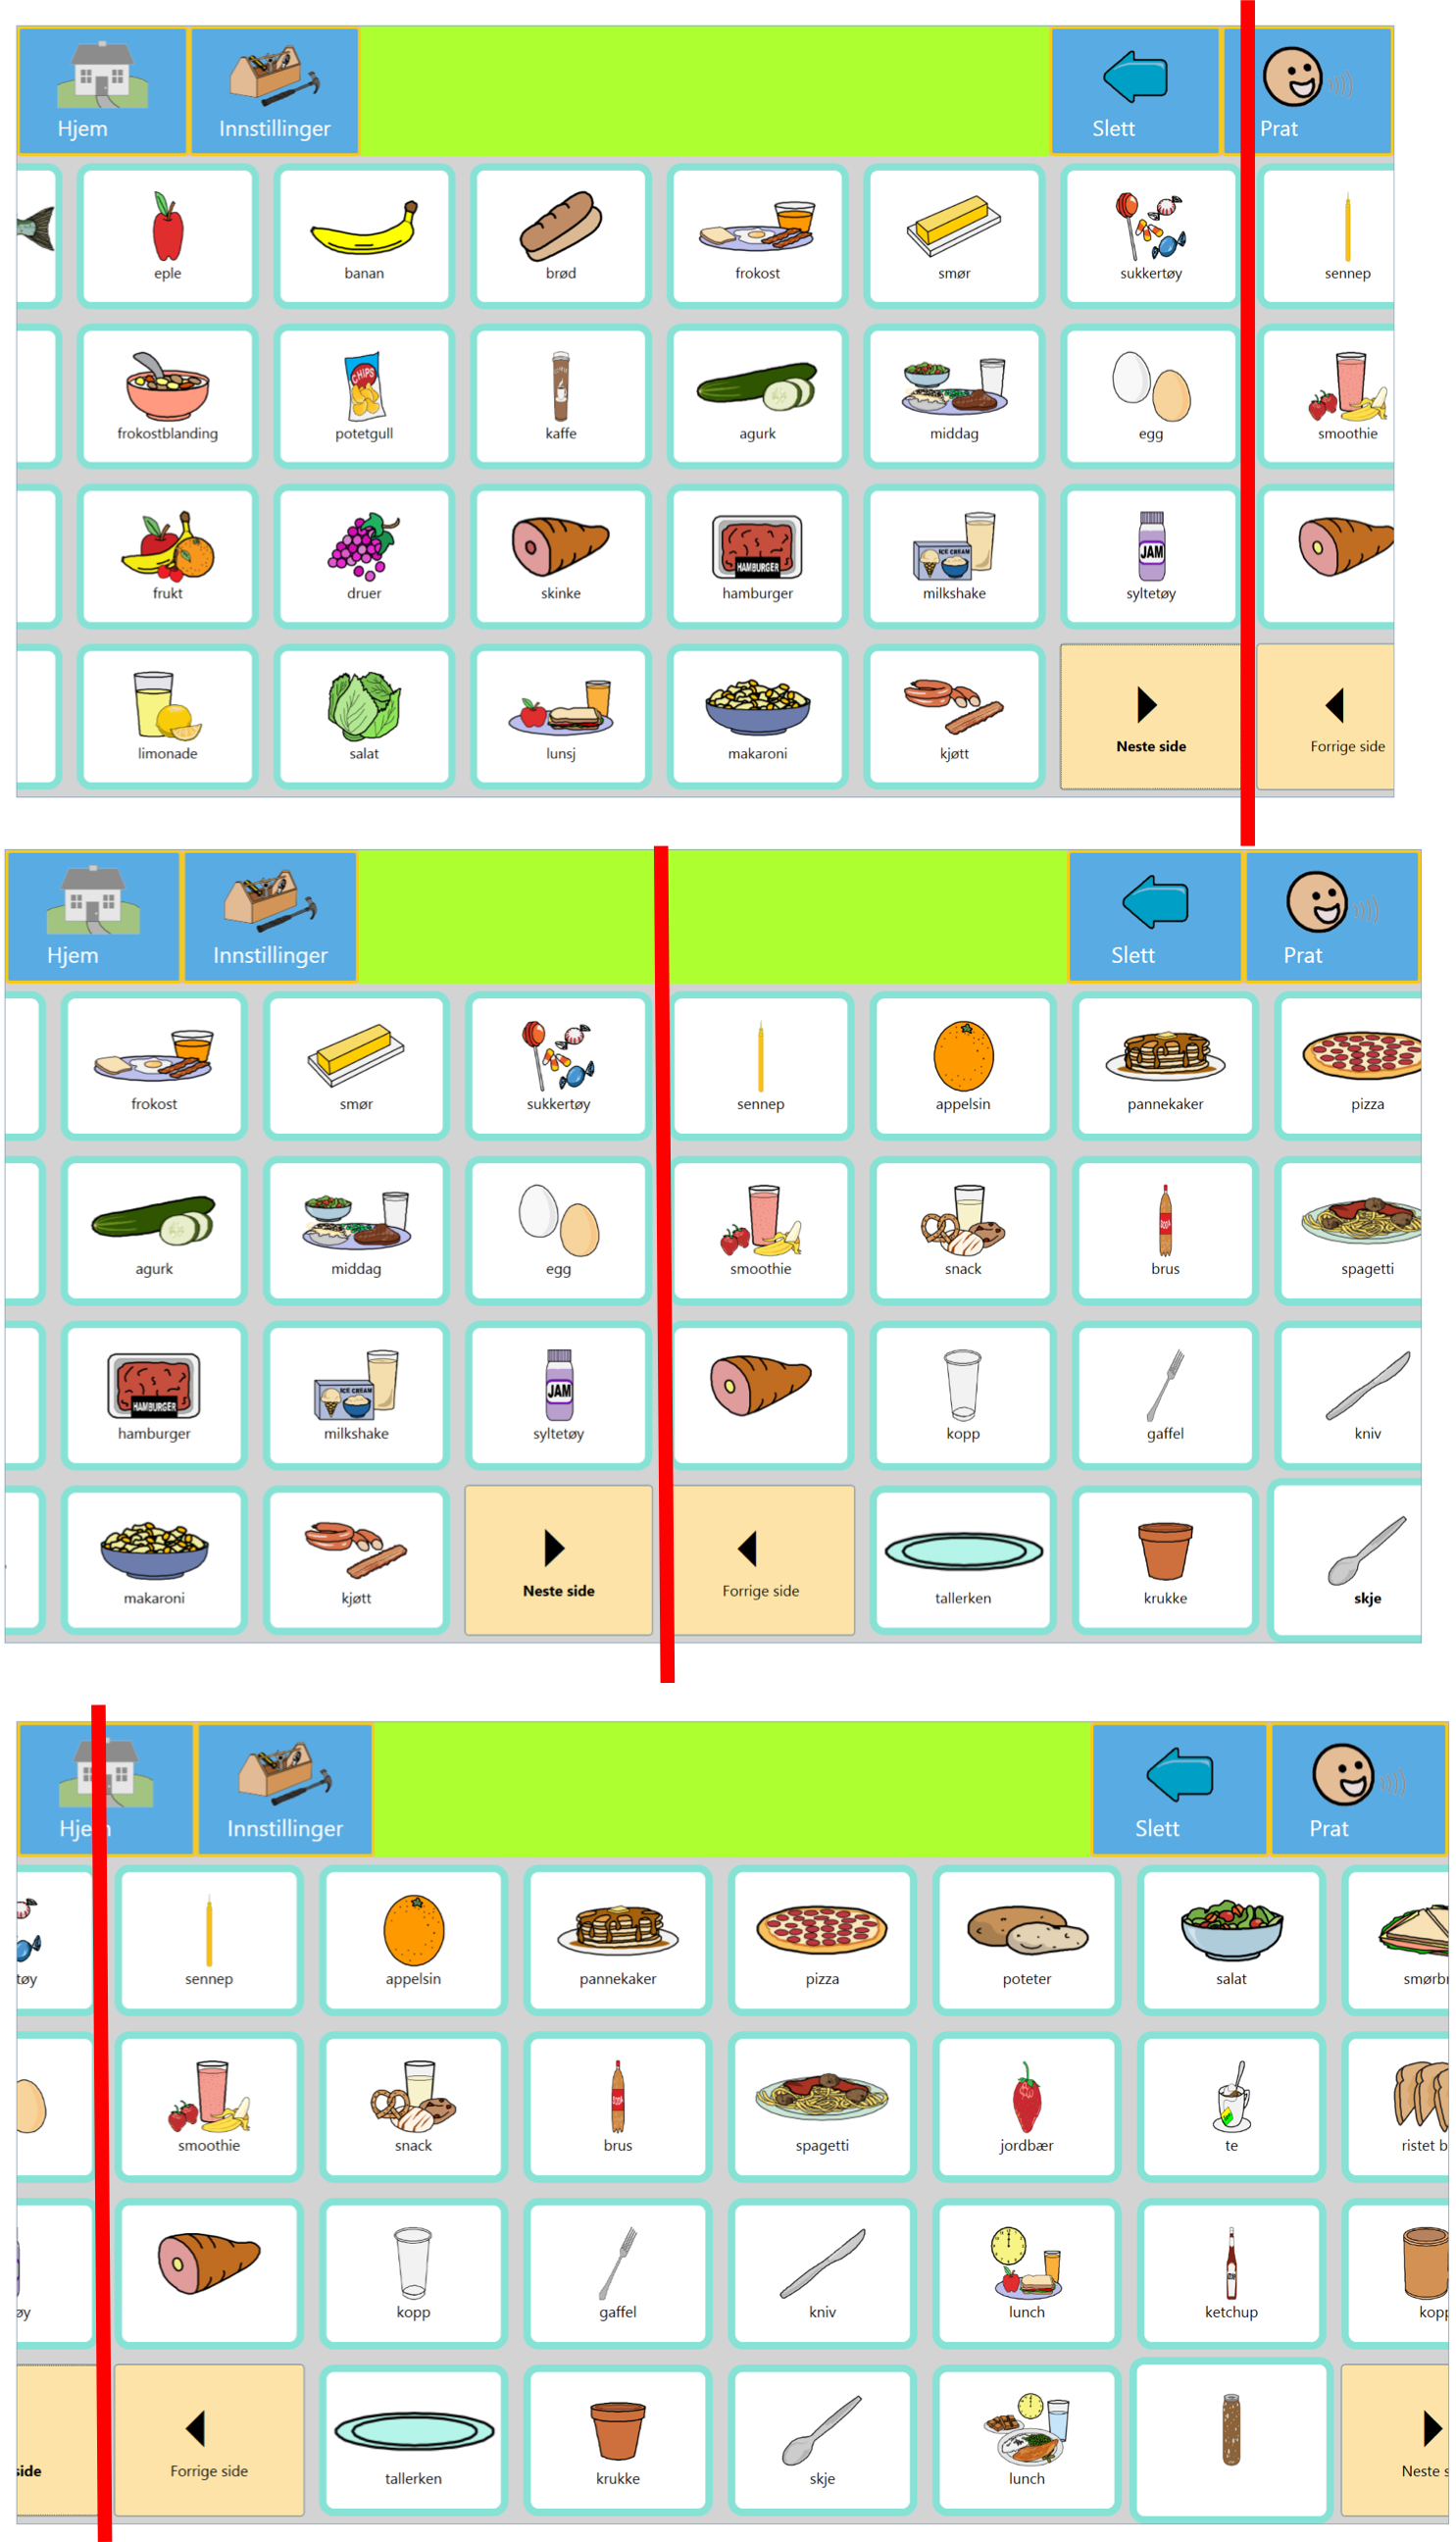
\includegraphics[height=18cm,keepaspectratio]{Slide}
\caption{Smidig glide animasjon}
\label{fig:navAni}
\end{figure}



\section{Lydeffekter} 
 
Som en del av rapporten ønsket vi å undersøke hvilken påvirkning lydeffekter hadde på brukeren. Hovedsakelig var målet å finne ut to ting. I hvilken grad hjelper effektene brukeren i å navigere rundt i applikasjonen og om det vil påvirke brukerens helhets uttrykk av applikasjonen.
 
 
\subsection{Lydeffekter i prototypen} 
 

I prototypen er det lagt til flere lydeffekter, utelukkende i form av små lydklipp på maks 1 sekund. Effektene vil kun bli avspilt som en respons til noe brukeren foretar seg eller for å informere om en hendelse. Denne begrensning finnes for ikke å skape forvirring hos brukeren. Hvis lyd også hadde blitt avspilt tilfeldig så ville meningen med effektene forsvinne, fordi brukeren blir lurt til å tro at programvaren har registrert en interaksjon, selv om han ikke har foretatt seg noe. Det er derfor viktig at det er lett for brukeren å skille mellom effektene som representerer en interaksjon og informasjon. 

De ulike interaksjonslydeffektene er også forskjellige, og hvilken som blir spilt er avhengig av,  som med animasjon,  hvilken type komponent brukeren samhandler med. Eksempelvis vil lyden som blir avspilt når brukeren trykker å tilbaketasten representere noe som forsvinner. De ulike lydene vil ikke bli beskrevet, fordi det fort kunne blitt absurd. 
 
 
 
\section{Brukertilpasning / Innstillinger}

For at en bruker skal kunne tilpasse prototypen etter egne preferanser, må han først trykke på knappen "innstillinger" i menylinjen. Han vil da bli navigert  til siden vist i figur \ref{fig:fart}, hvor han kan tilpasse farten til animasjonene som er brukt i prototypen. På siden vil de blå sirklene bevege seg med den hastighet de representerer, slik at brukeren får et inntrykk av farten. Fra figuren kan man se at det foreløpig kun er seks elementer som kan tilpasses.


\begin{figure}
\centering
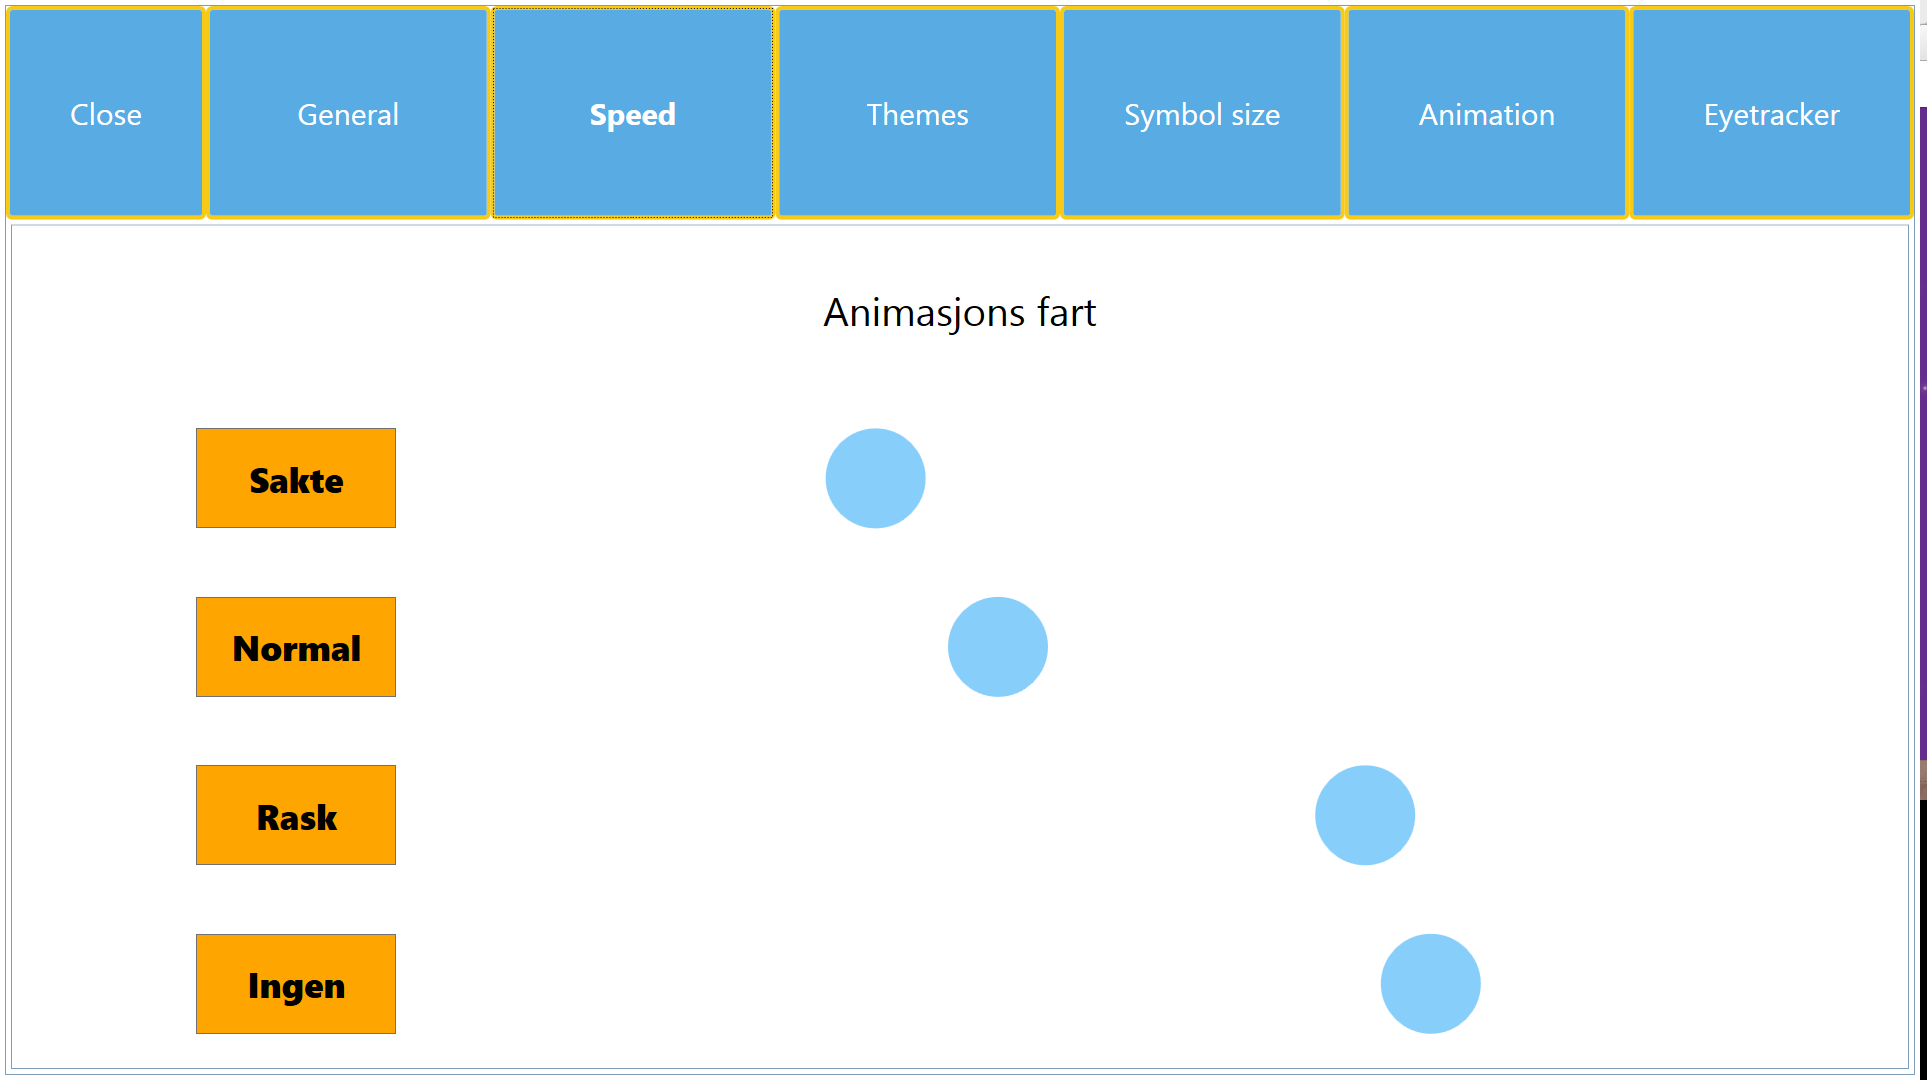
\includegraphics[width=16cm,keepaspectratio]{Fart}
\caption{Animasjonsfart innstillinger}
\label{fig:fart}
\end{figure}

En annen innstilling som brukeren kan endre på, er fargepaletten, kalt tema. I figur \ref{fig:my_label1} og \ref{fig:my_label2} vises de to temaene som er implementert i prototypen. Et hvor fargene er hentet fra tv-serien "powerpuff" og et fra serien "Turtles". Disse kan ikke være med i et sluttprodukt på grunn av opphavsrettigheter, men viser hvordan det kan løses. Ved å velge et av temaene vil fargene i prototypen endres deretter.

\begin{figure}
\centering
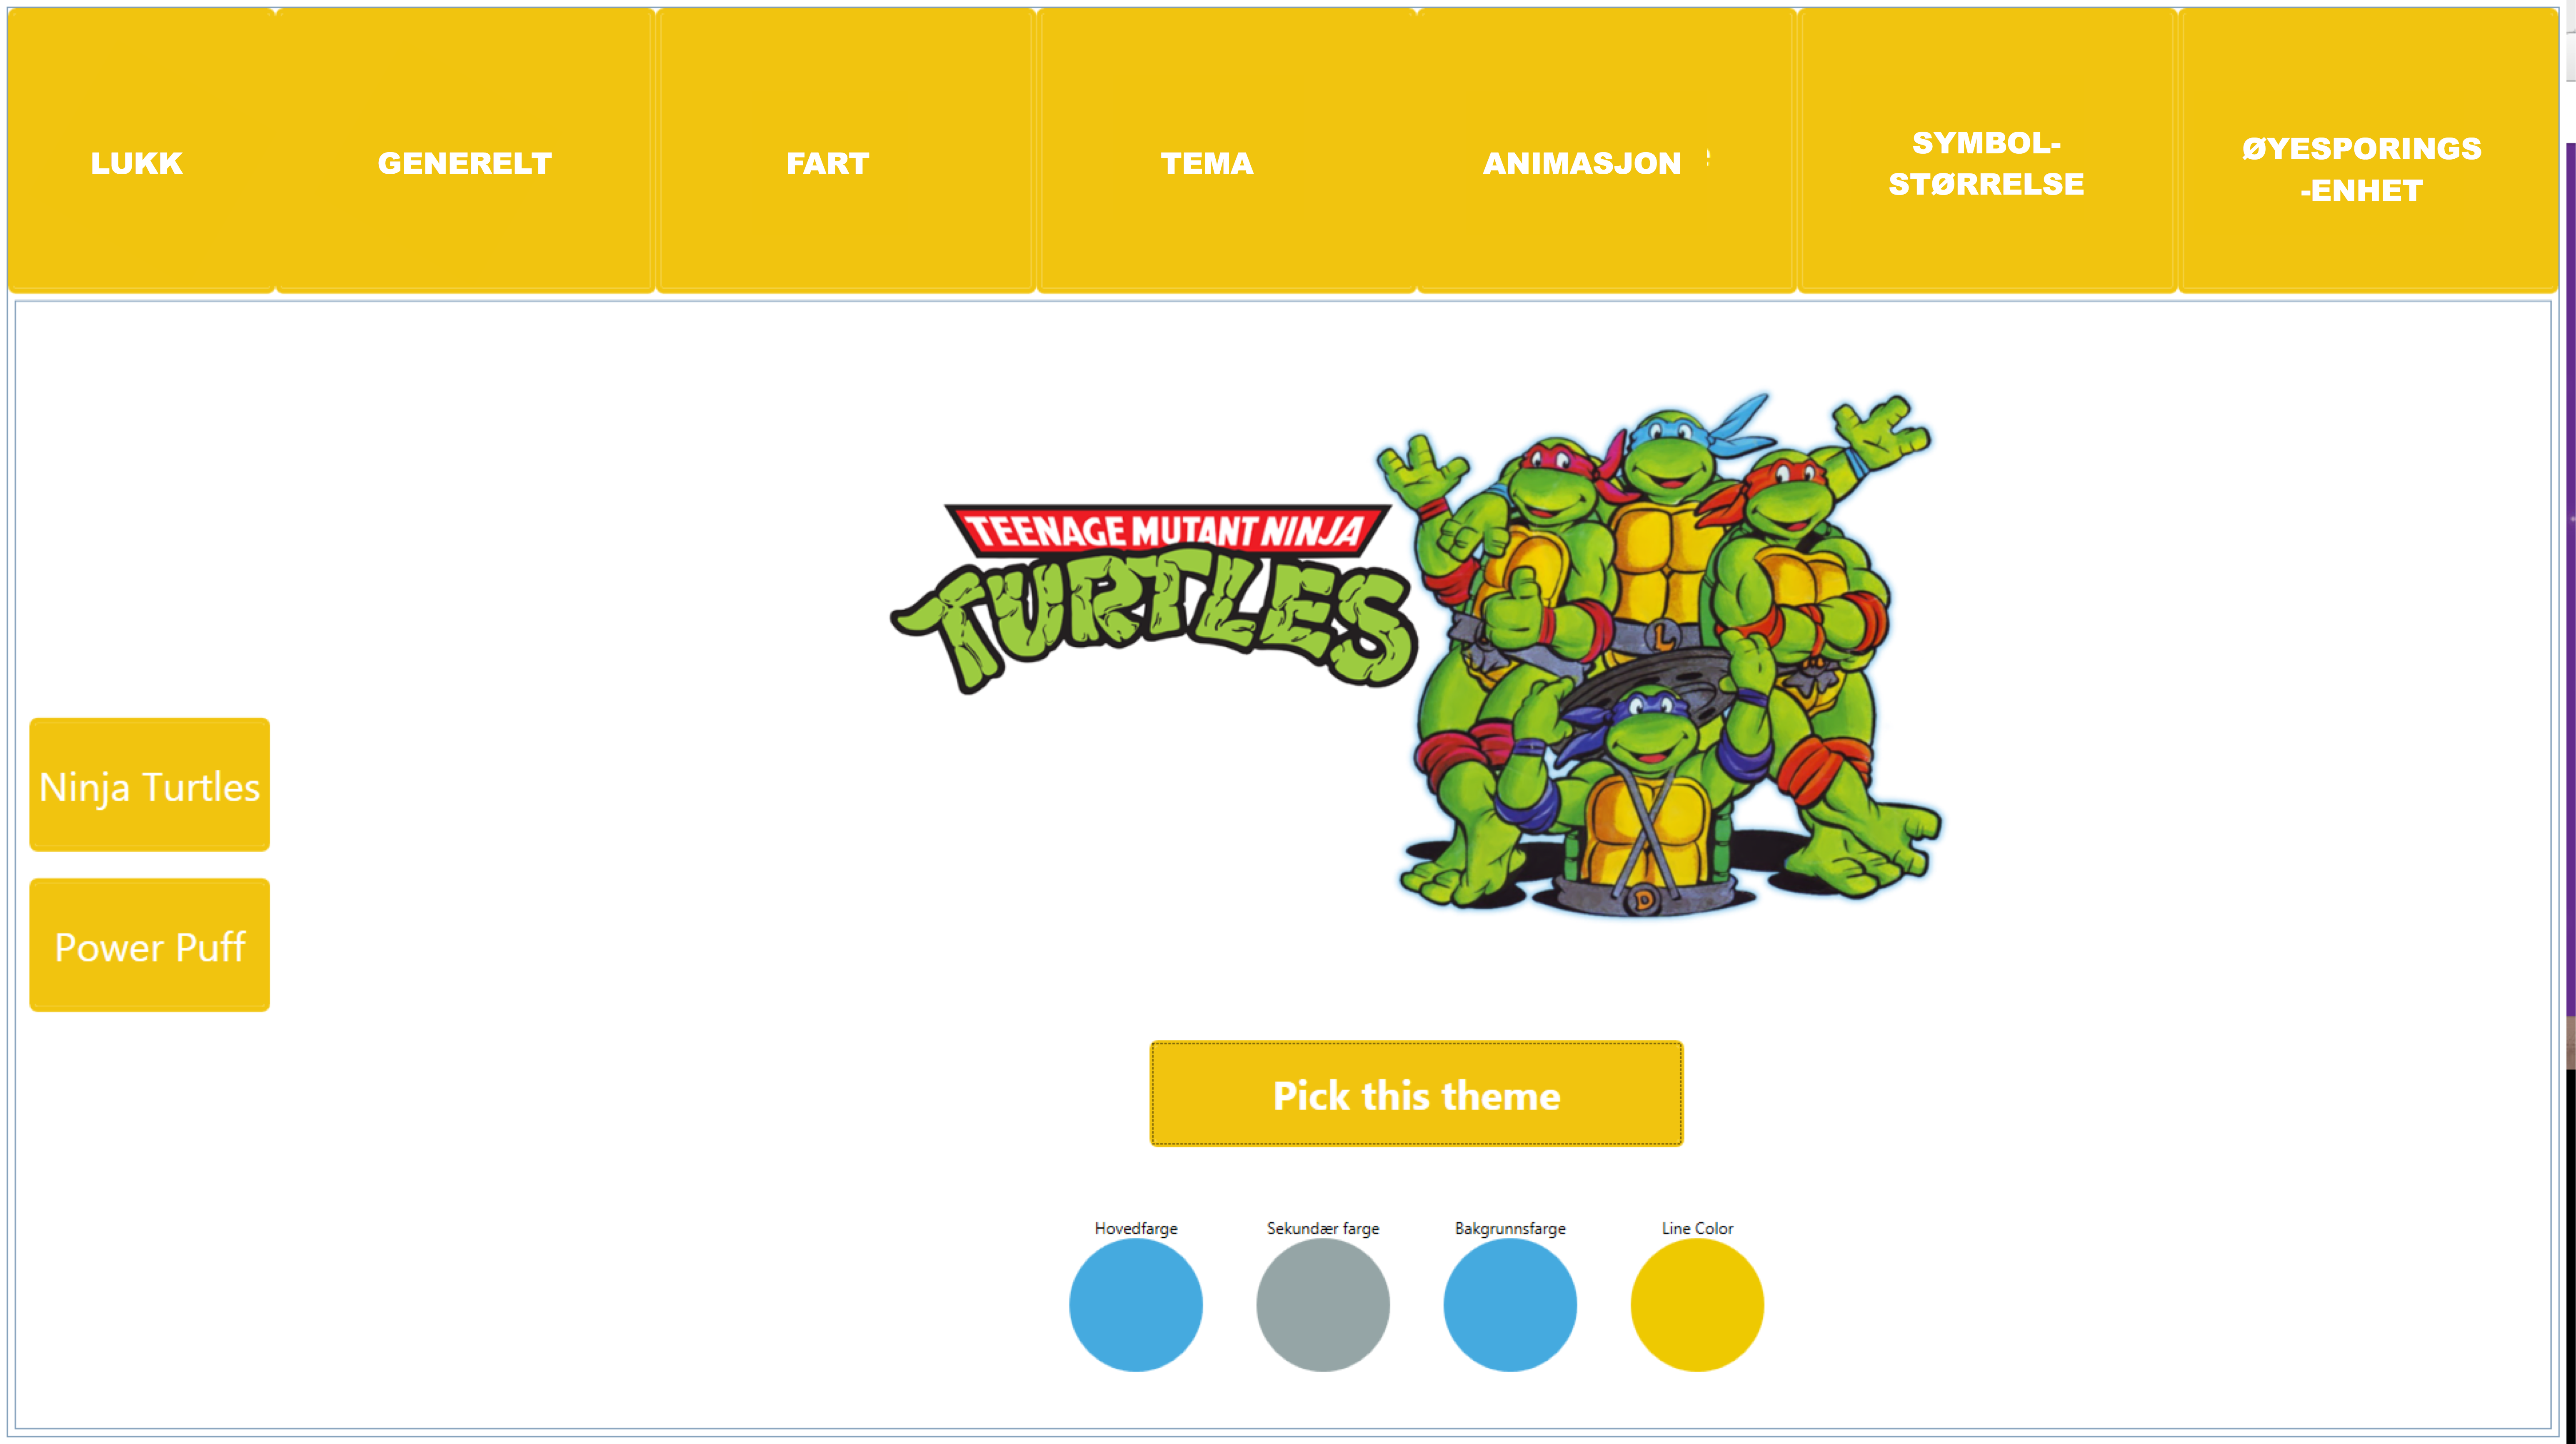
\includegraphics[width=16cm,keepaspectratio]{turtles1}
\caption{Ninja Turtles fargepalett }
\label{fig:my_label1}
\end{figure}

\begin{figure}
\centering
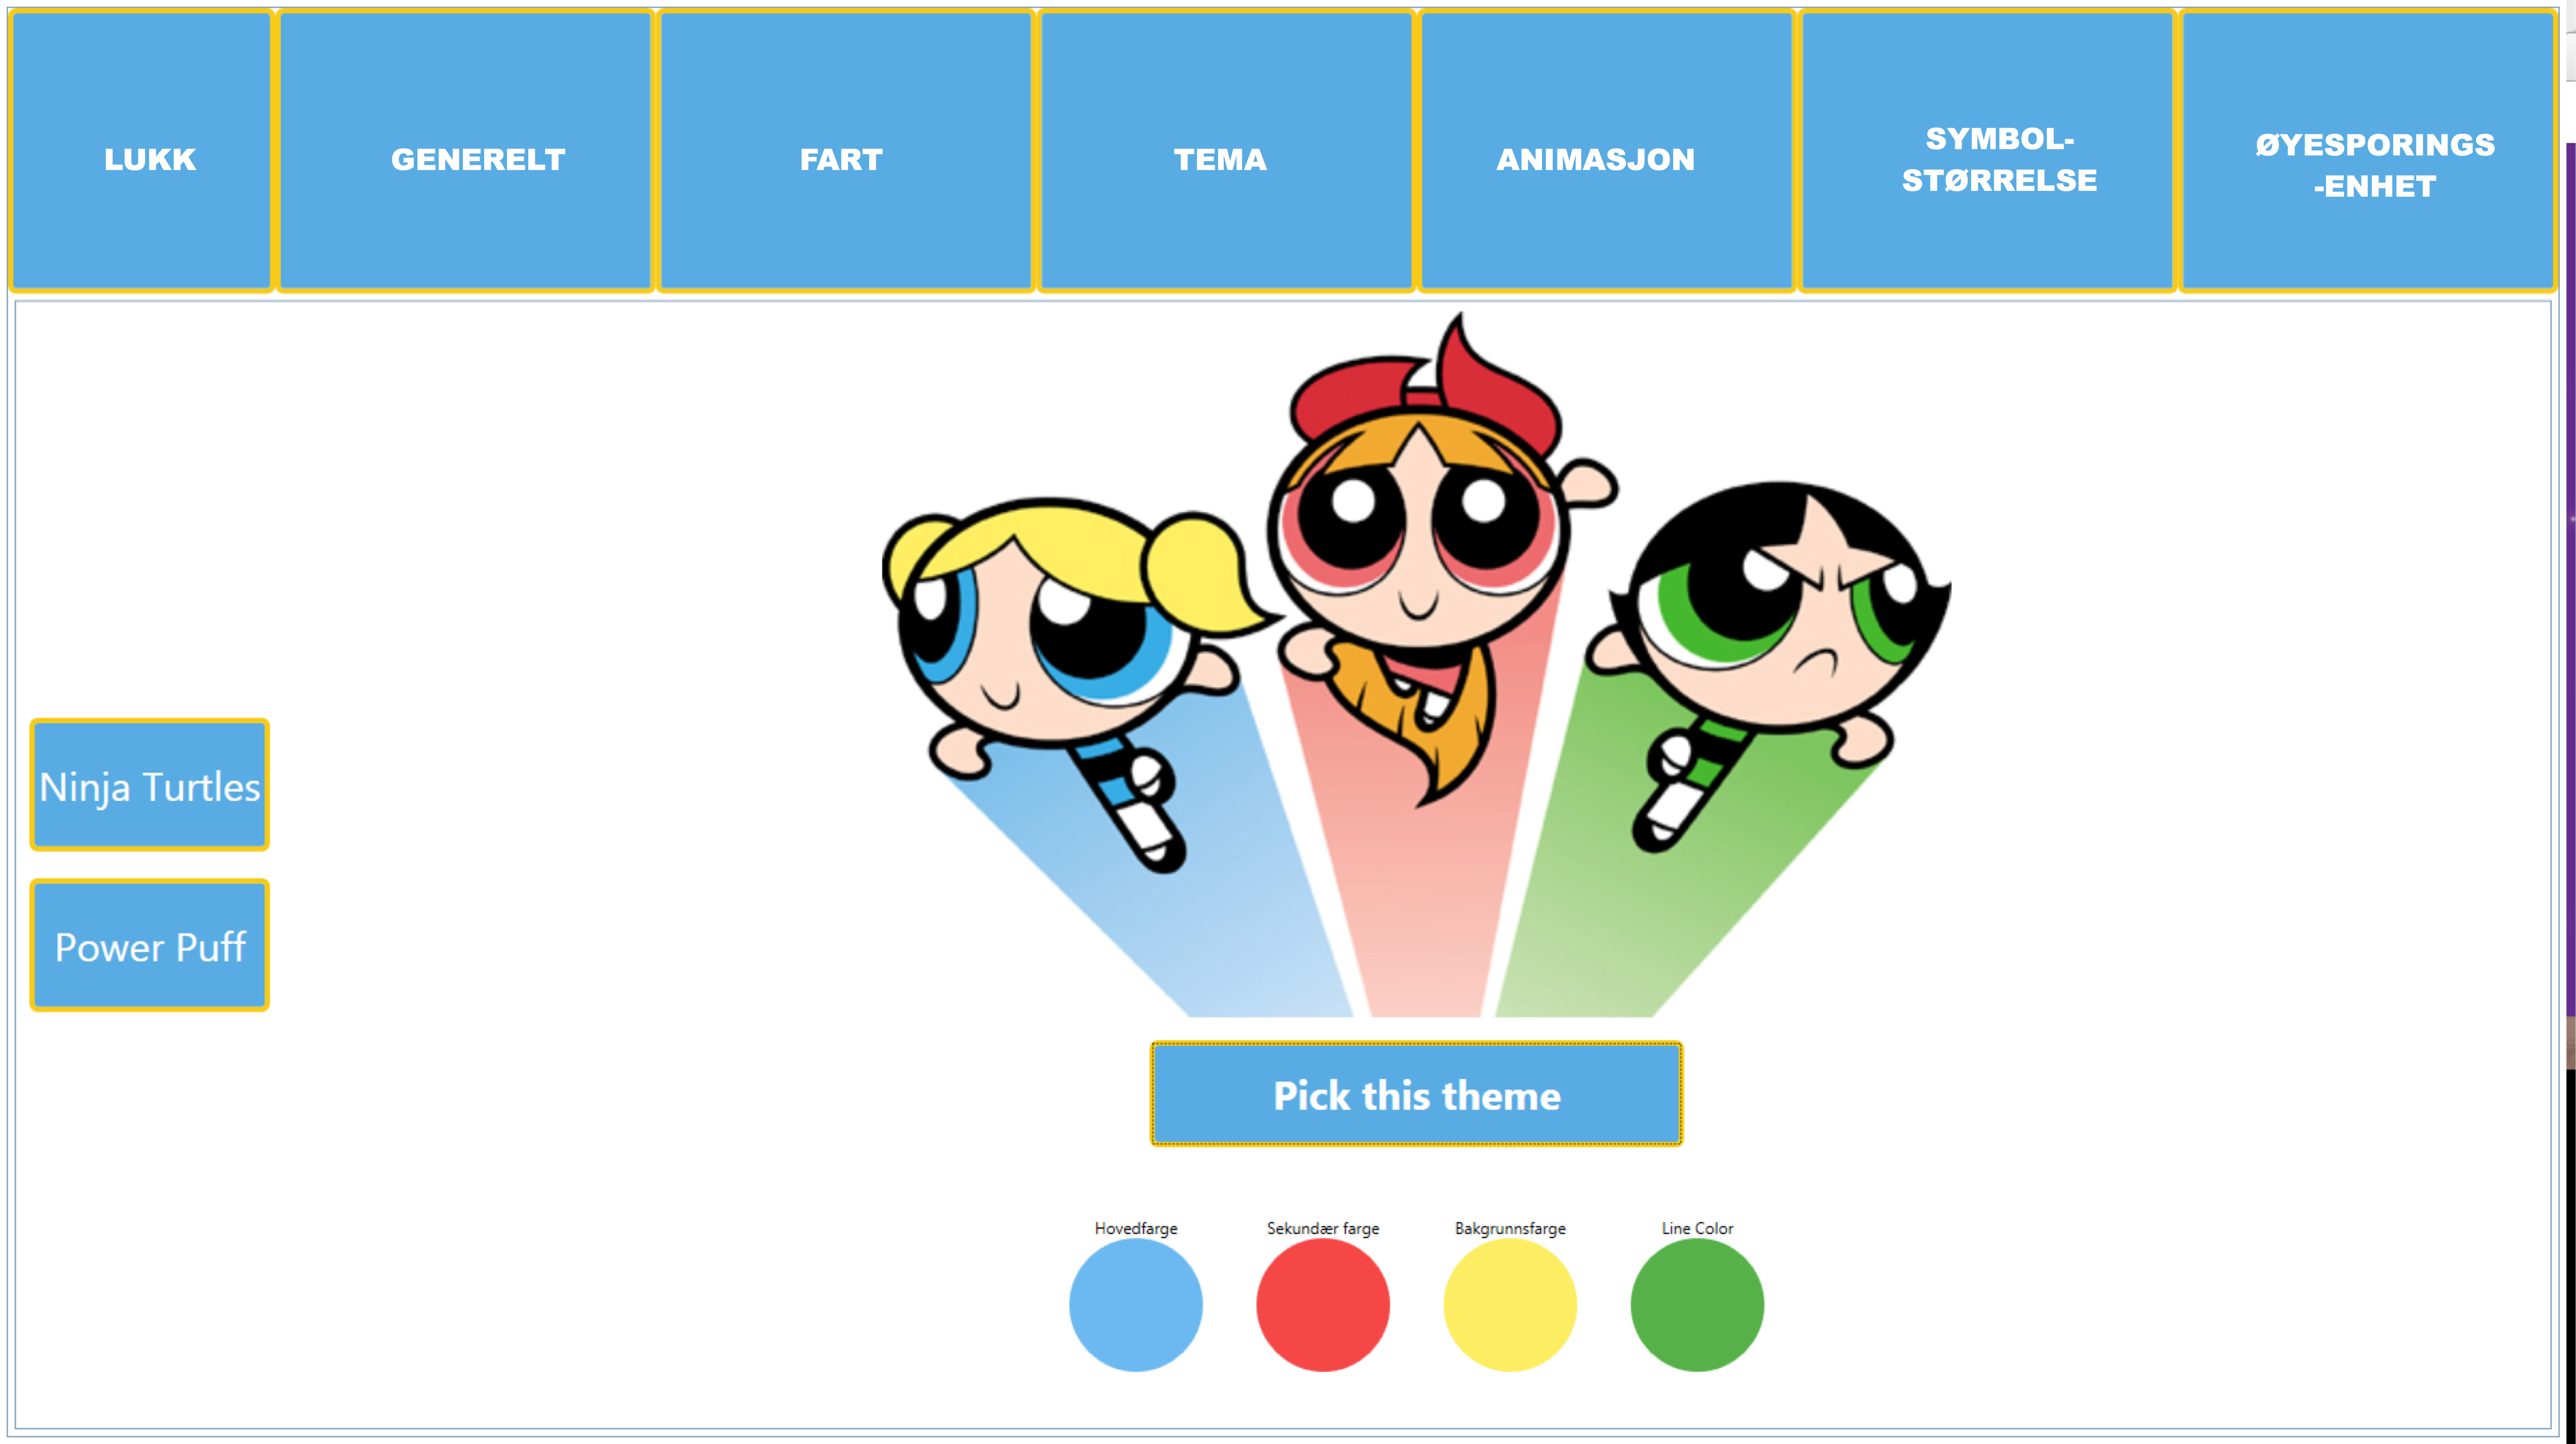
\includegraphics[width=16cm,keepaspectratio]{powerpuff1}
\caption{Powerpuff fargepalett }
\label{fig:my_label2}
\end{figure}


Når en bruker har endret på innstillinger er det greit at disse holder seg slik neste gang applikasjonen kjøres. For å holde innstillingene mellom kjøringer brukes en .NET tjeneste kalt Brukerinnstillinger \cite{Using812:online}. Dette gjør at ulike brukere på samme maskin kan ha forskjellige innstillinger, fordi den baserer seg på bruker og ikke på applikasjon.

